%%%%%%%%%%%%%%%%%%%%%%%%%%%%%%%%%%%%%%%%%%%%%%%%%%%%%%
%
% Where we discuss the code management infrastructure that is needed
% to support the analysis efforts 
%%%%%%%%%%%%%%%%%%%%%%%%%%%%%%%%%%%%%%%%%%%%%%%%%%%%%%

\chapter{Code management} % Tom Junk main editor
\label{chap:codemgt}

The DUNE experiment consists of several large components -- prototypes, a beam, a near detector, and a far detector,
which have their own schedules and subsets of the collaboration that work on them.  Computer simulation is used to
help optimize the design of the components in the early phases, and as an integral part of the analysis procedures
during the extraction of physics results.  Triggering, reconstruction and event selection all require sophisticated
software developed by teams over long time periods.  The large, international
collaboration introduces its own challenges regarding software development, deployment, and maintenance.
This section describes the software stacks in use on DUNE and some of which are expected in the future,
as well as technologies used to build, distribute, and maintain and archive the software.

\section{DUNE Software Stacks}

Commonality is sought among the several detector simulation and reconstruction efforts in order to maximize the
value of the several detectors planned for DUNE.  Liquid-argon time projection chambers (LArTPCs) are used in the 35-ton
prototype, the 3x1x1 dual-phase prototype, the single-phase and dual-phase ProtoDUNE detectors, 
one component of the near detector (a pixel-based
LArTPC), and the single-phase and dual-phase far detector (FD) modules.  Several other LArTPC's have operated or will
in the near future:  ICARUS, ArgoNeuT, LArIAT, MicroBooNE, SBND, and MiniCaptain, as well as some smaller prototypes,
such as LongBo, TallBo, CDDF, ArgonCube.  The LArSoft collaboration supports common software solutions for the
many LArTPC's and constitutes a large portion of DUNE software.  This section also describes some of the other
software stacks in use on DUNE, such as the beam simulation and triggering and DAQ.

\subsection{Beam Simulation}

The beam simulation software, G4LBNF, is based on GEANT4 and private code that defines the baffle, target, horn,
decay pipe, and shielding geometries and materials.  The geometry is specified in C++ methods so that parameters
can be adjusted algorithmically in order to optimize the beamline components.  This simulation is used to provide
standard flux predictions for downstream analyses, including near and far detector simulations, as well as
sensitivity projections.  It is also used to predict systematic uncertainties.  The hadronic interaction uncertainties
are estimated using the PPFX~\cite{ppfx} package, and focusing uncertainties are estimated by adjusting 
beamline component locations, horn current fields, and beam size, position, and angle offsets.  Additional
uncertainties, such as the thickness of the cooling water layer are included.  These predictions are provided
in TTree objects for simulated neutrinos and their progenitors for the flux predictions, as well as aggregate
prediction histograms and covariance matrices which provide a convenient interface for those not requiring the
full information in the TTrees.  Separate flux predictions and uncertainties are provided for the near and far
sites, due to geometrical effects.

\subsection{Triggering and DAQ}

The ProtoDUNE-SP and 35-ton detector data acquisition systems'
software is based on {\it artdaq}, a full-featured package that provides
for configuration control, interprocess communication, data ingestion, event building, logging, and monitoring.
The {\it artdaq} software is written and maintained by a dedicated group at Fermilab.  Experiment-specific plug-ins,
such as the boardreaders, are maintained by the DUNE DAQ group.  {\bf FIXME say something about ProtoDUNE-DP DAQ.}
The triggering for ProtoDUNE-SP is accomplished with an FPGA on the Penn Trigger Board which takes input from
the beam instrumentation components. 

Beam instrumentation data is stored in the DIP/DIM databases at CERN and extracted in near real-time by a dedicated
process, which stores a persistent version of the data for downstream merging with the detector data.

For DUNE, the intention is to use the IFBEAM database to communicate beam parameters such as bunch current
and arrival time at the target for later analysis.

\subsection{LarSoft}

LArSoft is a software toolkit based on the {\it art} event-processing framework.  It is used, developed, and
shared by many collaborations that use LARTPC detectors.  It speeds the development of simulation and reconstruction
software through this sharing, and also reduces the maintenance cost as software that is tested on one
experiment can be re-used on another, reducing the need for debugging and tuning, though some detector-specific
tuning remains in many cases.  LArSoft also provides definitions of commonly used data products, such as raw digits,
deconvoluted waveforms, hits, clusters, tracks, showers, vertices, and identified particles.

LArSoft is divided into several repositories, each of which contains the source code to build multiple shared
object libraries, and associated configuration and parameterized data files.  A user may check out one repository
at a time and set up pre-built versions of all of the others.  A dependency diagram is shown in 
Figure~\ref{fig:swdeptree}, headed by the DUNE-specific package {\tt dunetpc}.

\begin{figure}
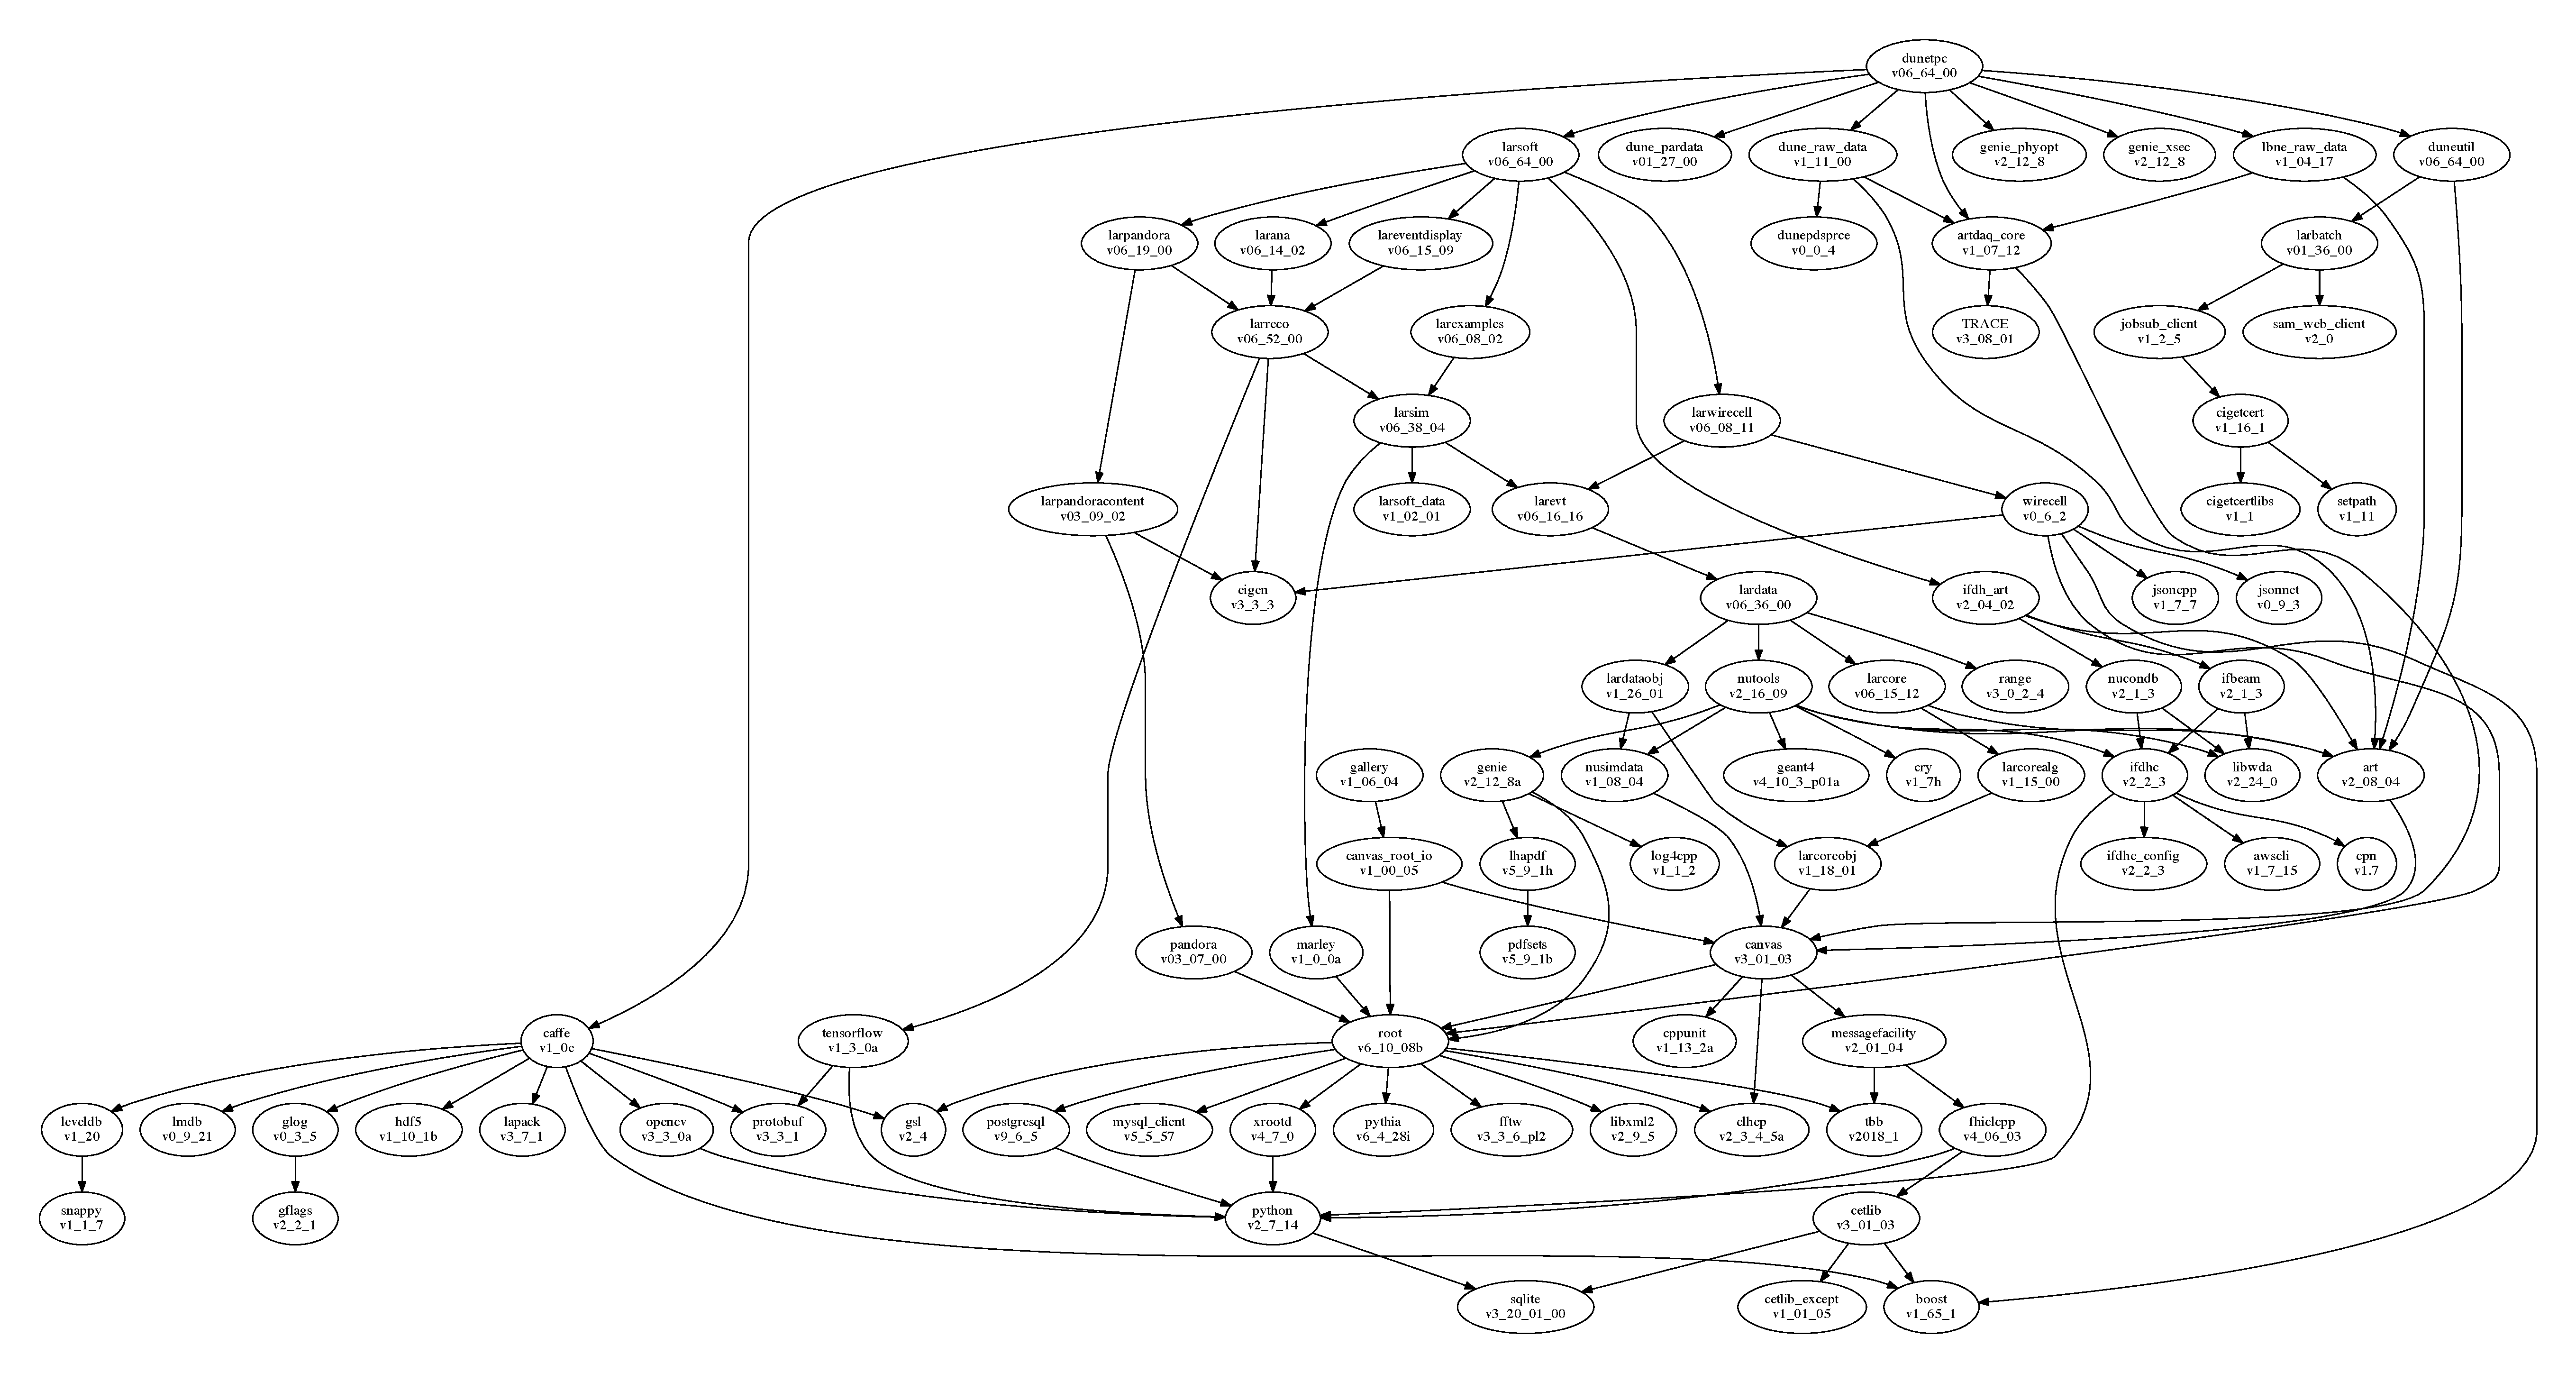
\includegraphics[width=0.95\textwidth]{software-computing/figures/dtree.pdf}
\caption{\label{fig:swdeptree} Software dependency tree for {\tt dunetpc}, showing dependent software products.}
\end{figure}

\subsubsection{Detector Simulation}

The detector simulation is based on GEANT4.  Detector geometry is read in from GDML files.  A common interface to
the GEANT4 stepping process simulates the details of the interaction of particles with liquid argon.  Once
the ionization energy has been determined by GEANT4, the fraction that recombines and makes light is computed
in LArSoft-specific routines (NEST or a simple parameterization).  The drift, diffusion, and attachment of electrons
on impurities are simulated in LArSoft code, as is the collection on the wires or pixels.  Detector electronics
response functions are provided by detector-specific parameterizations, as is noise, digitization, and compression.
The wrapped induction-plane wires provides a DUNE-specific challenge -- multiple wire segments are read out by
any given induction-plane DAQ channel.  LArSoft assumes that experiment-provided methods give the mapping between
DAQ channels and wire segments, and DUNE provides these for 35-ton, ProtoDUNE-SP, and the FD.  Parameters
such as the electric fields, argon temperature, electron lifetime, and others are specifiable in FHiCL files
that allow easy reconfiguration of a program without recompiling.

\subsubsection{Reconstruction}

Reconstruction proceeds in several steps.  The raw digits are uncompressed, stuck bits interpolated over,
noise filtered (coherent in space, frequency-based filtering in time), and the field response is deconvoluted,
an important step for optimizing the signal analysis from induction-plane wires.  Hits are fit as Gaussian
pulses to the filtered, deconvoluted waveforms.  A similar set of steps is used in the photon detector data
preparation.  Hits are grouped into clusters, which may be part of tracks or showers.  Several track-finding
and shower reconstruction algorithms have been developed.  Ones in common use on DUNE are the Projection-Matching
Algorithm (PMA)~\cite{PMA}, Pandora~\cite{Pandora}, and WireCell~\cite{wirecell}.  
PMA tests 3D hypotheses by projecting them onto the  2D plane (wire vs. time) of the observed data and 
testing the consistency.  Pandora builds up a 3D interpretation
of each event based on matching clusters in the 2D views, using a variety of algorithms tuned to specific topologies.
Pandora is in fact a framework into which simpler algorithms can be plugged in.  Pandora can be run in two modes:
cosmic-ray identification and rejection, and neutrino-scatter reconstruction.  These two modes were motivated by
MicroBooNE's needs, as each MicroBooNE trigger contains several cosmic-ray tracks on average.  FIXME how many?
The ProtoDUNE analyses will require similar steps in order to separate beam particle interactions from those
made by cosmic rays.  A convolutional neural network (CNN)
has been trained to identify hits as belonging to tracks or to showers based on neighboring pixels in the 
deconvoluted 2D data~\cite{CNN}.  Photon detector hits are grouped into flashes which are associated with
TPC clusters for further analysis.  The WireCell package is a tool that forms a three-dimensional image of the
event based on the raw digits.  It contains a two-dimensional deconvolution method that is able to use
the extra information that neighboring wires provide in order to extract more information about the signal on
a wire.  This 2D deconvolution has been shown to improve the identification and reconstruction of tracks that
travel in the plane of the electric field and an induction-plane wire.


The output files of the reconstruction contain data products made at all levels: raw and fitered/deconvoluted
digits, hits, clusters, tracks and particles, and associations between them.  It is necessary to keep this information
for purposes of reconstruction algorithm development and tuning, though production of large data sets may
drop the input data in the output files in order to reduce the storage requirements.  A ntuple format has bee
defined, called AnaTree, which provides convenient access to pertinent reconstructed information without
having to read the much larger {\it art}-formatted files.  The {\tt gallery} package~\cite{gallery} also provides
a simpler interface to reading {\it art}-formatted files from ROOT or Python scripts, or user-compiled standalone
programs.

\subsection{LArSoft-Like Software Packages}

Not all detector components on DUNE use LArSoft directly, though there is a strong motivation to use the
same framework and similar data products from one detector technology to another, in order to reduce the
overhead of learning new systems when collborators switch projects within DUNE, or even come from other
experiments to work on DUNE.  For example, {\tt hisoft} is a repository of code that simulates and reconstructs
events in the CDR reference design near detector, a straw-tube tracker in a magnetic field with a calorimeter
and muon chambers.  It is built on {\tt art} like LArSoft and has ported many of the features of LArSoft, but
does not use LArSoft directly.

\subsection{QScan}

QScan~\cite{QScan}  is a software package developed initially for ICARUS but which is now in use for the
dual-phase 3x1x1 prototype, ProtoDUNE-DP, and the proposed dual-phase FD module(s).  It provides the similar
functionality of simulation and reconstruction as LArSoft.  It is designed to be run in the online monitor
of ProtoDUNE-DP.  Reconstruction of ProtoDUNE-DP data with LArSoft is planned.

\subsection{External Software}

DUNE encourages the exploration and use of external simulation and reconstruction packages that are
publicly available.  One notable example is the ALICE full software stack~\cite{ALICEsw} which is used in the Gaseous
Argon TPC near detector simulation effort.  Another is the re-use of HighLAND, an ntuple-analysis tool
developed for T2K.  Some software, such as GeGeDe and EdepSim, have been developed with DUNE in mind
but are sufficiently general that they find use beyond the collaboration and are stored in GitHub instead
of a DUNE-controlled repository.

\section{Software Repositories}

Official (i.e. supported, maintained, version-controlled and archived) software is stored in git repositories
hosted at Fermilab.  The Redmine~\cite{redmine} web tool provides an html-based interface to each repository,
allowing developers to view current and previous versions, branches, commit comments and differences, and
annotated versions of the code indicating the person who checked in each line.  Redmine also provides wiki
support for associated documentation.  Automated code documentation systems such as DOxygen~\cite{DOxygen}
and LXR are in use.  Software checked in to the repositories should contain DOxygen-friendly headers and
specify the authors of the code.  The repositories are publicly visible without credentials.  In order to
modify software in a repository, however, permission must be granted by the DUNE software management team
to each developer.

In addition to {\tt dunetpc} which contains LArSoft-related code, there are {\tt duneutil} for utility scripts
and XML files used in production, and dune-raw-data (and lbne-raw-data) which contain DAQ interface software.

\subsection{Build Environment}

Most DUNE software is written in C++ which must be compiled and installed before it can be run.  We use the
Multi-Repository Build System {\tt MRB}~\cite{mrb}.  It is capable of managing a local release of many checked-out
git repositories' worth of code.  The smallest unit of code that can be checked out and compiled is the git
repository with MRB.  Other tools allow building smaller pieces.  MRB produces UPS products~\cite{ups} 
and installs them in a separate directory owned by the user.  It also can produce tarfiles containing
the built code arranged as a UPS product so it can be installed in a public location or transferred to a grid job.

The fact that the repository is the smallest unit of buildable code means that each repository needs to be
tagged with a version, and if code in one repository depends on code in another repository, then the
repository that requires the setup of the other one must also contain a file with the appropriate version numbers
of all dependent repositories.  In order for disk usage to be minimized and build times reduced, the sizes 
of the repositories must be made as small as practical.  The maintenance of versions and the effort
needed to factorize code that has grown in size provides pressure in the other direction.

\subsection{Software Environment Setup}

Code that uses UPS to set up depends on the environment variable LD\_LIBRARY\_PATH (on MacOS, the corresponding
variable is called DYLD\_LIBRARY\_PATH), which is a search path to find shared-object libraries.  This
variable is used by the image activator to load the desired pre-built code.  In the common case that a user
would like his or her own version of a shared library, the local version is in a directory earlier in the
search path than the publicly installed version, allowing convenient building and testing of small components
without rebuilding the entire application.  When UPS sets up a software product (for LArSoft, each git repository
is built into a single UPS product), it also sets up corresponding dependent products for a consistent set.
GEANT4, GENIE, and ROOT are most often set up in this manner.  Users logging in without setting up the DUNE
environment have a ``clean'' system with just operating-system and user-defined variables, which can be very
valuable when debugging a complicated situation that depends on a user's setup.
A UPS product's setup table file also specifies additions to the search paths PATH, FW\_SEARCH\_PATH, and FHICL\_FILE\_PATH,
which are used to search for command-line executables, framework data files, and job configuration files.  Any
other variables required by the software are also set up at this stage.

The UPS model assumes that all versions of software that are needed by any user of a system are already present
in directories that can be searched for the appropriate version.  Centrally-managed systems with large
shared disks for storing software had been in use but more modern distributed tools scale better for DUNE's
requirements.  This software environment differs from commercial distribution systems (like RPM, yum, pip,
and others) because of the need for physics analyses to be able to reproduce their results.  If an analysis is
in its final stages and systematic uncertainties are being evaluated, users are not able to upgrade to a new
version of the software, even if it is better (has a better reconstruction for example).  Multiple users of a computer
system may be in various stages of analyses and require stable versions that differ from each other.  To this end,
every component of the software stack, including the compiler, is distributed as UPS products.

The dependence of code on (DY)LD\_LIBRARY\_PATH causes an issue with MacOS.  The System Integrity Protection (SIP)
feature introduced with MacOS version 10.11 prevents its use by subprocesses when it is defined in a process.
The reasoning is that a malicious library can be placed earlier in a search path than a desired one and
cause a security breach.  While SIP can be disabled in MacOS versions 10.11 through 10.13, the LArSoft and
{\it art} development teams are not confident that this will persist indefinitely.  Furthermore, if Linux
distributions follow suit, then the use of library paths may become obsolete.

A future development in the bulid and setup systems is to use SpackDEV~\cite{SpackDEV}, which builds code in
a way that preserves the locations of the dependent libraries; these locations are stored in the calling
libraries' .so files at link time so that the operating system can insist that only the library that was used
at link time is the one used at run time.

\subsection{Code Distribution}

While the source code of DUNE's software stacks is publicly available, pre-built versions are needed
for running on grid computing resources, and also to speed development.  Pre-built binaries are distributed
along with the source code using CVMFS~\cite{CVMFS}, a distributed file system designed for efficient
distribution of code.  The source files and header files are needed for debugging and development,
even for other repositories that depend on a particular repository.  Pre-built binaries are distributed
for the major supported platforms:  Scientific Linux (currently SL6 and SL7), and MacOS (currently 10.11
and 10.12) are the supported platforms.  The distributed builds on Linux are built on nodes running
Scientific Linux Fermi, which is compatible with Scientific Linux CERN (SLC), CENTOS, and Red Hat Enterprise
Linux, with corresponding version numbers.  Other distributions of Linux are not currently supported.

Another distribution mechanism is a web server containing the pre-built binaries and source UPS products
collected in tarfiles.  These are stored at {\tt http://scisoft.fnal.gov}.  Along with the tarfiles are
files that contain lists of tarfiles needed to be downloaded in order to install a consistent set.

Each version of the code is provided with a debug build or with an optimize build.  Code compiled with
the optimizer turned on (FIXME -- O3?) is much faster than unoptimized code (some code runs four times faster
or more when optimized), but it is much more difficult to use with a debugger, due to out-of-order execution
of portions of statements, as well as the use of CPU registers for temporary variables, or removing some
calculations entirely.

\subsection{Release Management}

LArSoft and {\tt dunetpc} are large, distributed software efforts and frequently an upgrade to one product
requires a simultaneous upgrade to another.  Developers working with the latest source code of one repository
must then work with the latest source code of another repository.  In order to minimize the occurrence of this,
and allow developers to use pre-built binaries whenever possible, frequent releases of the LArSoft code stack
are made.  Each week, there is a release, and additional ones are made, as needed.

Because UPS sets up LArSoft when {\tt dunetpc} is set up, and only the matching version can be set up,
each week there is a release of {\tt dunetpc}, with a version number matching the LArSoft release.  Version
numbers contain three digits: major, minor, and patch numbers.  DUNE-specific code does not have to wait
for the weekly LArSoft release to make a DUNE release.  Adding additional identifying characters to a release
tag allows for multiple {\tt dunetpc} releases for each LArSoft release.

Frequently, changes in LArSoft require corresponding changes to {\tt dunetpc}, such as changing the directories
in which header files are located, when LArSoft undergoes a rearrangement.  These changes are frequently scripted
so that all experiments using LArSoft can upgrade easily.  Frequently developers of shared tools will make git
feature branches of changes that are required by their tool, and these feature branches are merged by the
DUNE software managers before tagging and building the weekly release.

Official releases are built on the Jenkins~\cite{jenkins} build system at Fermilab, which automates the
build process on all supported platforms and versions (such as debug or optimized builds).

\subsection{The {\it art} Framework}

DUNE's near and far detector simulation and reconstruction software, as well as that used for the ProtoDUNE
detectors, is built on LArSoft which is built on the {\it art} framework~\cite{art}.  The {\it art} framework
provides the event loop, I/O features not supported by ROOT such as parameterizable output file naming, configuration
using the Fermi Hierarchical Configuration Language (FHiCL), provenance storage by saving all configuration
information in the output file, message handling, and resource consumption (memory, CPU, I/O) accounting.  It
is supported by the {\it art} development team at Fermilab.  It provides the basis for both analysis programs
and for {\it artdaq}.  Extensive documentation and tutorials are provided~\cite{artdoc}\cite{arttutorial}.
The {\it art} deveopers hold weekly stakeholders' meetings at which experiment concerns and requests are aired.

\subsection{NTuple Analysis (CAFAna)}

The process of extracting oscillation parameters from DUNE's results requires a sophisticate fit to the near
and far detector data samples, using muon, electron, and possibly neutral-current candidate events.  This fit
must include the effects of detector acceptance and resolution, and also include systematic uncertainties on these.
The oscillation parameters affect predictions as functions of the true values $L/E$, while DUNE can only
measure an approximate energy on each event, so the full transfer function of true to measured energy must be
incorporated in the fits.  CAFAna~\cite{CAFAna} is a tool developed for use on NOvA, which takes as input
Monte Carlo and data NTuples and forms histograms in as many categories as the experiment defines, and performs
these fits.  It has been ported to DUNE to read similarly constructed NTuples built from fully-simulated
DUNE events.
